\section{Risks measures}

In this section we discuss different ways to measure the risk of portfolio.


\begin{definition}
	A portfolio with $n$ assets, $A_1, A_2, \dots, A_n$, is a vector $x^\top = (x_1, x_2, \dots, x_n)\in \R^n$ where each coordinate $x_i$ is the weight of capital invested in asset $A_i$.
\end{definition}

Let $L(x,y)$ be the loss associated with the decision vector $x$, to be chosen from a certain subset $X$ of $\R^n$ and the random vector $y \in \R^m$. The vector $x$ can be interpreted as representing a portfolio, with $X$ as the set of available portfolios
(subject to various constraints). The vector $y$ stands for the uncertainties, e.g. in market parameters, that can affect the loss. Of course the loss might be negative and thus, in effect, constitute a gain.

For each $x$, the loss $Y=L(x,y)$ is a random variable having a distribution in $\R$ induced by that of $y$. The underlying probability distribution of $y \in \R^m$ will be assumed to have density, which we denote by $p(y)$.

The probability of $L(x,y)$ not exceeding a threshold $\alpha$ is given by
\[
	\Psi (x,\alpha) = \int_{L(x,y)\leq \alpha} p(y)\,dy.
\]
As a function of $\alpha$ for fixed $x, \Psi(x, \alpha)$ is the \textit{cumulative distribution function} for the loss associated with $x$. Since $p(y)$ is continuous, $\Psi(x, \alpha)$ is nondecreasing with respect to $\alpha$ and continuous.


% The \textit{expected loss} $\mu$ of a portfolio $x$ is given by
% \[
% 	\mu(x) = \int_{y\in\R^m} L(x,y)\,p(y)\,dy.
% \]
% Moreover, the \textit{loss variance} of $x$ is
% \[
% 	\sigma^2(x) = \int_{y\in\R^m} \big(L(x,y)-\mu(x)\big)^2\,p(y)\,dy
% \]
% and the \textit{volatility} of the loss is $\sigma(x)$.

% The volatility of the loss was defined as a \textit{risk measure} to a portfolio by Nobel laureate in economics, Harry Markowitz in 1952 (see in \cite{Markowitz1952}) under the hypothesis of loss has a normal distribution. In the following we see that this choice is not the better one.

The probability of loss is a risk measure of a portfolio. However, in 1999 Artzner, Delbaen, Eber and Heath (see in \cite{Artzner1999}) defined, what they called \textit{coherent risk measure}, from the following axioms to a risk measure $\mathcal{R}$:


\begin{axiom}[Translation invariance] For all portfolio $x$ and all $m\in\mathbb{R}$,  we have
	\[
		\mathcal{R}(x+m) = \mathcal{R}(x)-m.
	\]
\end{axiom}
This means that adding an amount of cash, $m$, to a portfolio decreases your risk by the same amount.

\begin{axiom}[Subadditivity] If $x_A$ and $x_B$ are two portfolios, then
	\[
		\mathcal{R}(x_A+x_B) \leq \mathcal{R}(x_A) + \mathcal{R}(x_B),
	\]
\end{axiom}
In particular, this property means that ``a merger does not create extra risk.''

\begin{axiom}[Positive homogeneity] For all portfolio $x$ and all $\lambda\geq 0$ we have
	\[
		\mathcal{R}(\lambda x) = \lambda \mathcal{R}(x)
	\]
\end{axiom}
This property implies that the risk measure is a linear function of the size of the position.

\begin{axiom}[Monotonicity] Let $x_A$, $x_B$ be two portfolios,
	\[
		\mbox{if } x_A \prec x_B, \quad \mbox{then } \quad \mathcal{R}(x_A) \geq \mathcal{R}(x_B).\\
	\]
\end{axiom}
If a portfolio $x_A$ performs worse than $x_B$ in any
scenario $(x_A \prec x_B)$, then it means that the portfolio $x_A$ is
riskier than $x_B$.

\begin{definition}
	A risk measure satisfying the axioms of translation invariance, subadditivity, positive homogeneity, and monotonicity is called \textbf{coherent}.
\end{definition}


When the risk measure is not assumed to have variations proportional to the risk variations themselves, the positive homogeneity is no longer satisfied. Alternative axioms can be proposed.

\begin{axiom}[Convexity] For all portfolios $x_A$, $x_B$ and for all $0\leq \lambda \leq 1$,
	\[
		\mathcal{R}(\lambda x_A + (1-\lambda)x_A) \leq \lambda \mathcal{R}(x_A) + (1-\lambda) \mathcal{R}(x_B).
	\]
\end{axiom}

This axiom  was proposed in 2002 by Föllmer and Shield (see in \cite{Follmer2002}). It means that diversification does not increase risk.

\begin{definition}
	A risk measure satisfying the axioms of translation invariance, monotonicity, and convexity is called \textbf{convex}.
\end{definition}

\begin{proposition}
	A convex risk measure is coherent if it satisfies the positive homogeneity. Note also that the positive homogeneity and the subadditivity implies the convexity.
\end{proposition}

% The standard deviation does not satisfy translation invariance, however, this condition was defined with the perspective of banking system risk and is often ignored in case of portfolio construction.

In financial business, some of the risk management requirements are done in terms of loss distribution percentiles. An upper percentile of the loss distribution is called \textit{Value-at-Risk} ($\mbox{VaR}_\beta$)\footnote{By definition, $\mbox{VaR}_\beta$ is the percentile of the loss distribution, i.e., with a specified confidence level $\beta$, the $\mbox{VaR}_\beta$ of a portfolio is the lowest amount $\zeta$ such that, with probability $\beta$, the loss is less or equal to $\zeta$.}. For instance, $\mbox{VaR}_{0.95}$ is an upper estimate of losses which is exceeded with 5\% probability. The popularity of $\mbox{VaR}_\beta$ is mostly related to a simple and easy to understand representation of high losses. $\mbox{VaR}_\beta$ can be quite efficiently estimated and managed when underlying risk factors are normally (log-normally) distributed.

An alternatuve measure of losses is another percentile risk measure which is called \textit{Conditional Value-at-Risk} ($\mbox{CVaR}_\beta$). The $\mbox{CVaR}_\beta$ risk measure is closely related to $\mbox{VaR}_\beta$. For continuous distributions, $\mbox{CVaR}_\beta$ is defined as the conditional expected loss under the condition that it exceeds $\mbox{VaR}_\beta$, see Rockafellar and Uryasev (see \cite{RockafellarUryasev2001}). For continuous distributions, this risk measure also is known as \emph{Expected Shortfall}, \textit{Mean Excess Loss}, \textit{Mean Shortfall}, or \textit{Tail Value-at-Risk}.


\begin{figure}[H]
	\centering
	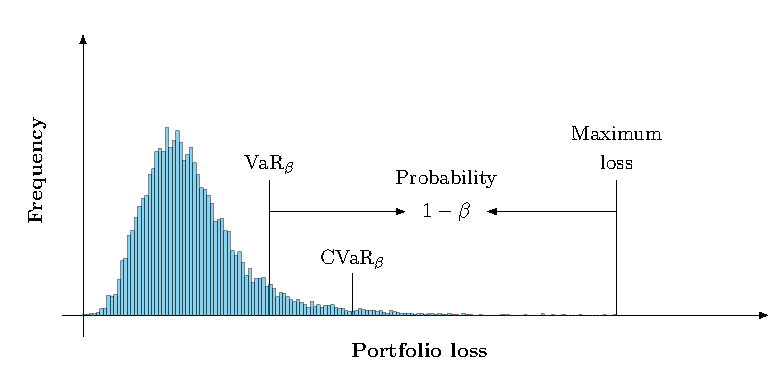
\includegraphics{figures/VarCvar.pdf}
	\caption{Portfolio Loss Distribution, VaR and CVaR}
	\label{fig:VarCvar}
\end{figure}

\begin{remark}\normalfont \hspace{1cm}
	\begin{itemize}
		\item The $\mbox{VaR}_\beta$ answers the question: what is the maximum loss with a specified confidence level $\beta$?
		\item The $\mbox{CVaR}_\beta$ answers the following question: what is the average loss in the $100(1-\beta)$\% worst case scenarios?
	\end{itemize}
\end{remark}

The $\mbox{VaR}_\beta$ and $\mbox{CVaR}_\beta$ values for the loss random variable $L(x,y)$ associated with $x$ and any specified probability level $\beta \in (0,1)$ will be denoted by $\alpha_\beta(x)$ and $\mbox{ES}_\beta(x)$. In our setting they are given by
\begin{equation}\label{eq:var}
	\alpha_\beta(x) = \min\{\alpha\in\mathbb{R} : \Psi(x,\alpha)\geq \beta \},
\end{equation}
and
\begin{equation}\label{eq:cvar}
	\mbox{ES}_\beta(x) = \frac{1}{1-\beta}\int_{L(x,y)\geq \alpha_\beta(x)} L(x,y)\, p(y)\,dy
\end{equation}

Although $\mbox{VaR}_\beta$ is a very popular measure of risk, $\mbox{VaR}_\beta$ is not a coherent risk measure as it does not satisfy subadditivity, but CVaR is a coherent risk measure.

Let $F_\beta:X\times \R \to \R$ be the function defined by
\[
	F_\beta(x,\alpha) = \alpha +\frac{1}{1-\beta}\int_{y\in\R^m}[L(x,y)-\alpha]^+ \, p(y)\, dy,
\]
where $[t]^+ = \max{t,0}$. The crucial features of $F_\alpha$, under the assumptions made above, are as
follows \cite[Theorem 2]{RockafellarUryasev2001}.

\begin{theorem}
	Minimizing the $\mbox{CVar}_\beta$ of the loss associated with $x$ over all $x\in X$ is equivalent to minimizing $F_\beta(x,\alpha)$ over all $(x,\alpha)\in X\times \R$, in the sense that
	\[
		\min_{x\in X}{\mbox{ES}_\beta(x)} = \min_{(x,\alpha)\in X\times \R}{F_\beta(x,\alpha)},
	\]
	where moreover a pair $(x^*, \alpha^*)$ achieves the right hand side minimum if and only if $x^*$ achieves the left hand side minimum and $\alpha^*\in A_\beta(x^*)$, where
	\[
		A_\beta(x^*) = \argmin_{\alpha\in \R}{F_\beta(x,\alpha)}.
	\]

	In particular, therefore, in circumstances where the interval $A_\beta(x^*)$ reduces to a single point (as is typical), the minimization of $F_\beta(x,\alpha)$ over $(x,\alpha)\in X\times \R$ produces a pair $(x^*, \alpha^*)$, not necessarily unique, such that $x^*$ minimizes the $\mbox{CVaR}_\beta$ and $\alpha^*$ gives the corresponding $\mbox{VaR}_\beta$.

	Furthermore, $F_\beta(x,\alpha)$ is convex with respect to $(x,\alpha)$ and $\mbox{ES}_\beta(x)$ is convex with respect to $x$, when $L(x,y)$ is convex with respect to $x$, in which case, if the constraints are such that $X$ is a convex set, the join minimization is an instance of convex programming.

\end{theorem}

\section{The Gaussian Case}

We now consider the case where the decision vector $x$ represents a portfolio of financial instruments in the sense that $x^\top = (x_1, x_2, \dots, x_n)$, with $x_i$ being the position in instrument $i$ and denoting by $y_i$ the return on instrument $i$, we take the random vector to be $y^\top=(y_1, y_2, \dots, y_n)$. The distribution of $y$ constitutes a joint distribution of the various returns and is independent of $x$; it has density $p(y)$.

The return on a portfolio $x$ is the sum of the returns on the individual instruments in the portfolio, scaled by the proportions $x_i$. The loss, being the negative of this, is therefore given by
\[
	L(x,y) = -[x_1y_1+x_2y_2+\cdots x_ny_n] = -x^\top y.
\]

As long as $p(y)$ is continuous with respect to $y$, the cumulative distribution function for the loss associated with $x$ will itself be continuous and although VaR and CVaR are usually defined in terms of monetary value, they could be defined as percentage returns the same happens to loss function.

For a closer look, let $\mu(x)$ and $\sigma(x)$ denote the mean and variance of the loss associated with portfolio $x$; in terms of the mean $\mu$ and variance $\Sigma$ of $y$, we have
\[
	\mu(x) = -x^\top \mu \quad \mbox{ and } \quad \sigma^2(x) = x^\top \Sigma x.
\]



% \begin{remark}\normalfont \hspace{1cm}
% 	\begin{itemize}
% 		\item The standard deviation does not satisfy condition 4, however, this condition was defined with the perspective of banking system risk and is often ignored in case of portfolio construction.
% 		\item VaR is not a coherent risk measure as it does not satisfy condition 1. This is a problem because the portfolio’s risk may have be meaningful in this case.
% 		\item CVaR is a coherent risk measure.
% 	\end{itemize}
% \end{remark}


We assume now that the random variable of loss $Y=L(x,y)$ is normally distributed, that is, $Y\sim N(\mu,\sigma^2)$. Let $\phi(z) = \frac{1}{\sqrt{2\pi}}e^{-z^2/2}$ be the probability density function of Standard Normal Distribution and $\Phi(x) = \int_{-\infty}^{x}\phi(z) dz$
the standard normal accumulated density function.

Since $P\big[L(x,y)\leq \alpha\big]= \Psi(x,\alpha)$, where $P\big[L(x,y)\leq \alpha\big]$ is the probability that loss is less than $\alpha$. By definition we have
$P\big[L(x,y)\leq \alpha_\beta(x)\big]=\beta$, which standardizing we obtain:
\[
	P\left[ \frac{L(x,y)-\mu(x)}{\sigma(x)} \leq \frac{\alpha_\beta(x)-\mu(x)}{\sigma(x)}
		\right]=\beta.
\]
Hence,
\[
	\frac{\alpha_\beta(x)-\mu(x)}{\sigma(x)}=\Phi^{-1}(\beta)
\] and then
\begin{equation}\label{eq:var2}
	\alpha_\beta(x)=\mu(x)+ \Phi^{-1}(\beta)\sigma(x).
\end{equation}

This is a special case of the standard deviation-based risk measure with $c = \Phi^{-1} (\beta)$. It implies that the value-at-risk is a coherent and convex risk measure if the asset returns are normally distributed. The expression of the expected shortfall is:

\[
	\mbox{ES}_\beta(x) = \frac{1}{1-\beta}\int_{\alpha_\beta(x)}^\infty y\, p(y)\,dy,
\] considering $p(y)$ the normal density function, we have that:
\[
	\mbox{ES}_\beta(x) = \frac{1}{1-\beta}\int_{-\mu(x)+ \sigma(x)\Phi^{-1}(\beta)} ^\infty \frac{y}{\sigma(x)\sqrt{2\pi}} e^{-\frac{1}{2}\big(\frac{y+\mu(x)}{\sigma (x)}\big)^2} dy,
\]

With the variable change
$t=\frac{y+\sigma(x)}{\sigma(x)}$, we obtain

\[
	\begin{aligned}
		\mbox{ES}_\beta(x) & = \frac{1}{1-\beta}\int_{\Phi^{-1}(\beta)}^\infty (-\mu(x)+ \sigma(x)t) \frac{1}{\sqrt{2\pi}} e^{-t^2/2}dt \\
		                   & = \frac{\mu(x)}{1-\beta}[\Phi(t)]_{\Phi^{-1}(\beta)}^\infty +
		\frac{\sigma(x)}{(1-\beta)\sqrt{2\pi}}\int_{\Phi^{-1}(\beta)}^\infty t e^{-t^2/ 2}dt                                            \\
		                   & =\mu(x) + \frac{\sigma(x)}{(1-\beta)\sqrt{2\pi}}\Big[-e^{-t^2/2} \Big] _{\Phi^{-1}(\beta)}^\infty          \\
		                   & = \mu(x) + \frac{\sigma(x)}{(1-\beta)\sqrt{2\pi}}e^{-\frac{[\Phi^{-1}(\beta)]^2}{2}}
	\end{aligned}.
\]

So CVaR can be calculated by
\begin{equation}\label{eq:cvar2}
	\mbox{ES}_\beta(x)=\mu(x) + \frac{\phi(\Phi^{-1}(\beta))}{1-\beta}\sigma(x).
\end{equation}
Like the value-at-risk, it is a standard deviation-based risk measure with $c ={\phi(\Phi^{-1}(\beta))}/{(1-\beta)}$
In the Gaussian world, different risk measures can be calculated using the expected return and volatility.

The volatility of the loss, $\sigma^2(x)$,  was defined as a risk measure to a portfolio by Nobel laureate in economics, Harry Markowitz in 1952 (see in \cite{Markowitz1952}) under the hypothesis of loss has a normal distribution. Note that, in this case,  by (\ref{eq:var2}) and (\ref{eq:cvar2}), that both Var and CVaR are the form $\mu(x)+c\sigma(x)$. In general, we want a portfolio with positive returns, that is, $\mu(x)\leq0$. If the portfolio manager has very optimistic forecasts, component $\mu(x)$ may substantially reduce the risk measure. This explains why omitting the mean component is standard practice in the asset management industry. Under the hypothesis of loss has a normal distribution volatility, VaR and CVaR are coherent risk measures.

\begin{example}\normalfont
	We consider three stocks $A$, $B$ and $C$ whose current prices are respectively $\$ 15.00$, $\$ 25.00$ and $\$ 30.00$. We assume that their expected returns are equal to $30$ bps\footnote{1 bps or one basis point is equivalent to
		0.01\% (the hundredth part of 1\%) or 0.0001 in decimal form.}, $50$ bps and $20$ bps on a daily basis and their daily volatilities are $3\%$, $2\%$, and $1\%$ respectively. The asset correlation matrix is given by
	\[
		\rho = \left(
		\begin{array}{rrr}
				1.00 & 0.40 & 0.15 \\
				0.40 & 1.00 & 0.60 \\
				0.15 & 0.60 & 1.00
			\end{array}
		\right)
	\]

	We consider a portfolio composed by $100$ stocks $A$, $200$ stocks $B$ and $100$ stocks $C$. The value of this portfolio is $\$ 9,500.00$, being $\$ 1,500.00$ invested in stock $A$, $\$ 5,000.00$ in stock $B$ and $\$ 3,000.00$ in stock $C$, therefore the weights of the stocks in this portfolio are $15.79\%$, $52.63\%$, and $31.58\%$ respectively, so $x=(0.1579;\;0.5263;\; 0.3158)$. The expected loss of the portfolio is $\mu(x) = -30\times0.1579+50\times0.5263+20\times0.3158$, that is, $\mu(x) = -37$ bps. Using the relationship $\Sigma_{i,j}=\rho_{i,j}\sigma_1\sigma_j$ we find the covariance matrix
	\[
		\Sigma = \left(
		\begin{array}{llr}
				9.0 & 2.4 & 4.5 \\
				2.4 & 4.0 & 1.2 \\
				4.5 & 1.2 & 1.0
			\end{array}
		\right)\times10^{-4},
	\] since the volatility of portfolio is given by $\sigma^2(x) = x^\top \Sigma x$, we have that $\sigma(x) = 1.51\%$.

	Considering $\alpha = 0.99$, we have $\Phi^{-1}(0.99) = 2.325$ and
	$\phi(\Phi^{-1}(0.99))=\phi(2.325)=2.68\%$. Using the equations
	$(\ref{eq:var2})$ and $(\ref{eq:cvar2})$ we have

	\[
		\begin{aligned}
			\mathrm{VaR}_{99\%}(x) & = -0.37\% + 2.325 \times 1.51\% = 3.14\%              \\
			\mathrm{ES}_{99\%}(x)  & = -0.37\% + \frac{2.68}{0.01} \times 1.51\% = 3.68\%.
		\end{aligned}
	\]

	Risk can also be expressed in monetary terms, in this case,

	\[
		\begin{aligned}
			\mathrm{VaR}_{99\%}(x) & = 3.14\% \times \$ 9,500.00 = \$ 298.30  \\
			\mathrm{ES}_{99\%}(x)  & = 3.68\% \times \$ 9,500.00 = \$ 349.60.
		\end{aligned}
	\]
	According to the result of {\rm VaR}, in $99\%$ of the days, the loss will be less than $\$ 298.30$, however in the $1\%$ of the remaining days the {\rm VaR} does not measure how much great can be the loss, this is the role of {\rm CVaR} which indicates that the average loss will be $\$ 349.60$ on the worst $1\%$ days.
\end{example}


\section{Portfolio optimization}

We consider a universe of $n$ assets. Let $x^\top = (x_1, x_2, \dots, x_n)$ be a portfolio and denoting by $R_i$ the return of asset $i$. If $R^\top=(R_1, R_2, \dots, R_n)$  is the random vector of asset returns then the return of portfolio $x$ is given by:
\[
	R(x) = [x_1R_1+x_2R_2+\cdots x_nR_n] = -x^\top R.
\]
If we note $\mu$ and $\Sigma$ the vector of expected returns and the covariance matrix of asset returns, we deduce that the expected return of portfolio $x$ is equal to:
\[
	\mu(x) = -x^\top \mu
\]
whereas its variance is given by:
\[
	\sigma^2(x) = x^\top \Sigma x.
\]
The mean-variance portfolio (MVP) of Markowitz (\cite{Markowitz1952}) consists in maximizing the expected return $\mu(x)$ for a fixed value $\sigma_0$ of the volatility $\sigma(x)$. This can be achieved by solving a standard quadratic programming (QP) problem:
\begin{eqnarray}\label{prob:MVP}
	\min_{x\in X} \,\, - \mu(x), \\
	\mbox{s.t. }\left\{
	\begin{aligned}\nonumber
		\sigma(x) = \sigma_0, & \\
		\mathbf{1}^\top x=1   &
	\end{aligned}
	\right.
\end{eqnarray}
where $\textbf{1}^\top =(1,1,\dots,1)$. The set of constraints $X$ could be defined by one or more properties, for example:
\begin{itemize}
	\item Capital constraint: $\textbf{1}^\top x=1$;
	\item Long-only constraint: $x\geq0$;
	\item Self-financial constraint: $\textbf{1}^\top x=0$;
	\item Holding constraint: $I\leq x\leq W$ where $I,W\in\R^n$ are lower and upper bounds of the asset positions, respectively.
	\item Leverage constraint: $\|x\|_1\leq K$.
\end{itemize}

The portfolio optimization is defined when we want to minimize (or maximize) a performance measure subject to a set of constraints. To performance measures there are, for example:

\begin{itemize}
	\item Expected return: $\mu(x)$;
	\item Volatility: $\sigma(x)$;
	\item Sharpe Ratio (SR): expected return per unit of risk
	      \[
		      SR = \frac{x^\top \mu - r_f}{\sigma(x)}
	      \]
	      where $r_f$ is the risk-free rate (e.g. interest rate on a Treasury bill);
	\item Information Ratio (IR): Sharpe Ratio with $r_f=0$;
	\item VaR (Value at Risk): quantile of the loss;
	\item CVaR (Conditional Value at Risk): expected value of the loss above some quantile.
\end{itemize}

We can choose a lot of optimization problems, like global minimum CVaR portfolio (GMCP)

\begin{eqnarray}\label{prob:GMCP}
	\min_{x\in X} \,\, ES_\beta(x), \\
	\mbox{s.t. }\left\{
	\begin{aligned}\nonumber
		\mathbf{1}^\top x=1   & \\
		\mathbf{0}\leq x \leq \mathbf{1}
	\end{aligned}
	\right.
\end{eqnarray}
 or 
\begin{eqnarray}\label{prob:GMCP2}
	\min_{x\in X} \,\, \lambda ES_\beta(x) - \mu(x) , \\
	\mbox{s.t. }\left\{
	\begin{aligned}\nonumber
		\mathbf{1}^\top x=1   & \\
		\mathbf{0}\leq x \leq \mathbf{1}
	\end{aligned}
	\right.
\end{eqnarray}
where $\lambda$ is a parameter that controls how risk-averse the investor is.


\section{Risk Parity}

Markowitz’s portfolio has never been fully embraced by practitioners, among other reasons because it only considers the risk of the portfolio as a whole and ignores the risk diversification (i.e., concentrates risk too much in few assets, this was observed in the 2008 financial crisis): one solution is the risk parity portfolio.

Risk parity is an approach to portfolio management that focuses on allocation of risk rather than allocation of capital. The risk parity approach asserts that when asset allocations are adjusted to the same risk level, the portfolio can achieve a higher Sharpe ratio and can be more resistant to market downturns.

While the minimum variance portfolio tries to minimize the variance (with the disadvantage that a few assets may be the ones contributing most to the risk), the risk parity portfolio distributes the weights so that the risk contribution of each asset (or asset class, such as bonds, stocks, real estate, etc.) is the same.

To define a risk-based allocation strategies it is necessary define how the risk of an asset affects the risk of the portfolio. 
Let $x^\top=(x_1,x_2,\dots,x_n)$ be a portfolio with $n$ assets and $\mathcal{R}(x)$ be a differentiable, homogeneous risk measure of $x$. Since $\mathcal{R}(x)$ is homogeneous, we have
\[
\mathcal{R}(x)=\frac{d}{d\lambda}\mathcal{R}(\lambda x)=\sum_{i=1}^n x_i \frac{\partial \mathcal{R} (x)}{\partial x_i}
\]
we can define the risk contribution of the asset $i$ by
$\mathcal{RC}_i$, where
\[
\mathcal{RC}_i(x)= x_i \frac{\partial \mathcal{R}(x)}{\partial x_i}.
\]
Therefore, the risk can be written as follows
\[
\mathcal{R}(x)=\sum_{i=1}^n \mathcal{RC}_i(x)
\]
which is known as \textbf{Euler's Allocation Principle}.

Volatility and $\mbox{CVaR}_\beta$  satisfy the properties required by the risk measure, $\mathcal{R}$, defined above. However, $\mbox{VaR}_\beta$ satisfies these properties only in the Gaussian case. When asset returns have a Normal Distribution, by simplicity (see Remark \ref{re:Normal}), we have that
$\mathcal{R}(x)=\sigma(x)=\sqrt{x^\top\Sigma x}$, it follows that
\[
\mathcal{RC}_i(x)= x_i \frac{\partial \sigma(x)}{\partial x_i}=\frac{x_i (\Sigma x)_i}{\sqrt{x^\top\Sigma x }}.
\]

It may be interesting for the investor to choose different risks for different assets, in this case the investor choose the percentage of risk that each asset should have in the portfolio, that is,
\begin{equation}\label{eq:RBP}
	\mathcal{RC}_i(x)=b_i\mathcal{R}(x),
\end{equation}
where $b_i$ represents the risk contribution that asset $i$ will have in the portfolio. Certainly $b_i\geq 0$ for all $i$ and
${\bf 1}^\top b =1$, with $b=(b_1, b_2, \dots, b_n)$. A portfolio distribution based in relation \eqref{eq:RBP} is called \textit{risk budgeting portfolio} (RBP), when $b_i=1/n$, for all $i$ the distribution is called \textit{risk parity portfolio} (RPP) or \textit{equal risk portfolio} (ERP).

In general, find the risk budgeting portfolio consists to solve the following non-linear system
\begin{eqnarray}\label{eq:SisNLin}
\mathcal{RC}_i(x)=b_i\mathcal{R}(x), \\
	\mbox{s.t. }\left\{
	\begin{aligned}\nonumber
b_i \geq 0, \\
x_i \geq 0, \\
{\bf 1}^\top b =1, \\
{\bf 1}^\top x =1.
	\end{aligned}
	\right.
\end{eqnarray}











Only in trivial cases can we find analytical solutions for this system, however, we can always find numerical solutions.

Consider $b^\top = (b_1, b_2, \dots, b_n)$, with ${\bf 1}^\top b =1$ and $f(x;b)$ defined by:
\[
f(x;b) = \sum_{i=1}^n \big(\mathcal{RC}_i(x) -b_i\mathcal{R}(x)\Big)^2
\] and the following optimization problem
\begin{eqnarray}\label{eq:MinProb}
\min_{x\geq \textbf{0}}\, \{f(x;b)\}; \\
	\mbox{s.t. }\left\{
	\begin{aligned}\nonumber
		\mathbf{1}^\top x=1 & \\
		\mathbf{0}\leq x \leq \mathbf{1}
	\end{aligned}
	\right.
\end{eqnarray}

If $x^\star$ is the solution to the problem (\ref{eq:MinProb}) and
$f(x^\star;b)=0$, so $x^\star$ is also system solution
(\ref{eq:SisNLin}). So we can use some optimization algorithm
quadratic to find a solution to the PDR. as it was
said before, to find a PPR just choose $b_i=1/n$, in the
process of choosing a PDR.

In the Gaussian case, when asset returns have a Normal distribution, we can consider $\mathcal{R}(x)=\sigma(x)$ and the system (\ref{eq:SisNLin}) reduces to
\begin{eqnarray}\label{eq:SisGauss}
x_i (\Sigma x )_i = b_i x^\top \Sigma x,\\
	\mbox{s.t. }\left\{
	\begin{aligned}\nonumber
b_i \geq 0, \\
x_i \geq 0, \\
{\bf 1}^\top b =1, \\
{\bf 1}^\top x =1.
	\end{aligned}
	\right.
\end{eqnarray}
for $i=1,2,\dots,n$.


Setting $w=x/\sqrt{x^\top \Sigma x}$, the equation $x_i (\Sigma x )_i = b_i x^\top \Sigma x$ is equivalent to $w_i(\Sigma w)_i =b_i$, or, in vector form
\[
\Sigma w = b/w.
\]

In 2013, Spinu (see in \cite{Spinu2013}) showed that the convex function
\[
f(w)= \frac{1}{2}w^\top \Sigma w - b^\top log(w)
\]
has a gradient equal to
\[
\nabla f(w) = \Sigma w - b/w
\]
and the system (\ref{eq:SisGauss}) can be reformulated by the following optimization problem
\begin{eqnarray}\label{eq:GaussProb}
\min_{x\geq {\bf 0}}\,\Big\{\frac{1}{2}w^\top \Sigma w - b^\top \log(w)\Big\};  \\
	\mbox{s.t. }\left\{
	\begin{aligned}\nonumber
		\mathbf{1}^\top x=1 & \\
		\mathbf{0}\leq x \leq \mathbf{1}
	\end{aligned}
	\right.
\end{eqnarray}


whose optimality condition is $\nabla f(w) = 0$ or $\Sigma w = b/w$ which is precisely the solution of the system (\ref{eq:SisGauss}).




